\documentclass[11pt]{article}

\usepackage{amsmath}
\usepackage{graphicx}
\usepackage{subcaption}

\newcommand{\numpy}{{\tt numpy}}    % tt font for numpy

\topmargin -.5in
\textheight 9in
\oddsidemargin -.25in
\evensidemargin -.25in
\textwidth 7in

\begin{document}

% ========== Edit your name here
\author{Aobo Yang (ay6gv)}
\title{CS6316: HW1}
\maketitle

\medskip

% ========== Begin answering questions here
\begin{enumerate}

\item
Linear Algebra Review

1.1

$$ x_1=-1,\, x_2=0,\, x3=1 $$

1.2

$$
A = \begin{bmatrix}
    2 & 2 & 3 \\
    1 & -1 & 0 \\
    -1 & 2 & 1
\end{bmatrix},
\:
b = \begin{bmatrix}
    1 \\
    -1 \\
    2 \\
\end{bmatrix}
$$

1.3

$$
\begin{bmatrix}
    2 & 2 & 3 \\
    1 & -1 & 0 \\
    -1 & 2 & 1
\end{bmatrix}\begin{bmatrix}
    c_1 \\
    c_2 \\
    c_3 \\
\end{bmatrix} = \begin{bmatrix}
    0 \\
    0 \\
    0 \\
\end{bmatrix}
$$

Since $(c_1, c_2, c_3) = (0, 0, 0)$, the columns are linearly independent

The rank of $A$ is $3$
\medskip

1.4

$$
A^{-1} = \begin{bmatrix}
    1 & -4 & -3 \\
    1 & -5 & -3 \\
    -1 & 6 & 4
\end{bmatrix}
$$

$$
det(A)= (2 \times -1 \times 1) + (3 \times 1 \times 2) - (3 \times -1 \times -1) - (2 \times 1 \times 1) = -1
$$

1.5
$$x = A^{-1}b = \begin{bmatrix}
    1 & -4 & -3 \\
    1 & -5 & -3 \\
    -1 & 6 & 4
\end{bmatrix}\begin{bmatrix}
    1 \\
    -1 \\
    2 \\
\end{bmatrix}=\begin{bmatrix}
    -1 \\
    0 \\
    1 \\
\end{bmatrix}$$

1.6

$$
\langle x,\, b \rangle = -1 \times 1 + 0 \times -1 + 1 \times 2 = 1,
$$

$$
x \otimes b = \begin{bmatrix}
    -1 \times 1 & -1 \times -1 & -1 \times 2 \\
    0 \times 1 & 0 \times -1 & 0 \times 2 \\
    1 \times 1 & 1 \times -1 & 1 \times 2
\end{bmatrix}=\begin{bmatrix}
    -1 & 1 & -2 \\
    0 & 0 & 0 \\
    1 & -1 & 2
\end{bmatrix}
$$

1.7

$$ L_1= |1| + |-1| + |2| = 4 $$
$$ L_2= (1^2 + (-1)^2 + 2^2)^\frac{1}{2} = \sqrt{6} $$
$$ L_\infty = 2 $$

1.8

$$
A_1 = \begin{bmatrix}
    2 & 2 & 3 \\
    1 & -1 & 0 \\
    -1 & 2 & 1 \\
    -1 & 2 & 1
\end{bmatrix},
\:
b = \begin{bmatrix}
    1 \\
    -1 \\
    2 \\
    1
\end{bmatrix}
$$

1.9

The rank is $A_1$ is also $3$
\medskip

1.10

No, this cannot be solved. Because the last two equations has conflicts. $-x_1+2x_2+x_3$ cannot both be $2$ and $1$.
\medskip

1.11

$$
A_1^+ = \begin{bmatrix}
    1 & -4 & -1.5 & -1.5 \\
    1 & -5 & -1.5 & -1.5 \\
    -1 & 6 & 2 & 2
\end{bmatrix}
$$

1.12

Yes, $B$ is orthogonal matrix because $B^TB=I$
\medskip

1.13

$$ \frac{\partial (y^TAy)}{\partial y} = y^T(A + A^T)$$


\item
Linear Regression Model Fitting

2.2

The initial data plot after \texttt{load\_data\_set()} is shown in Figure \ref{fig:data}.
\medskip

\begin{figure}[!h]
    \centering
    \begin{subfigure}[b]{0.4\linewidth}
      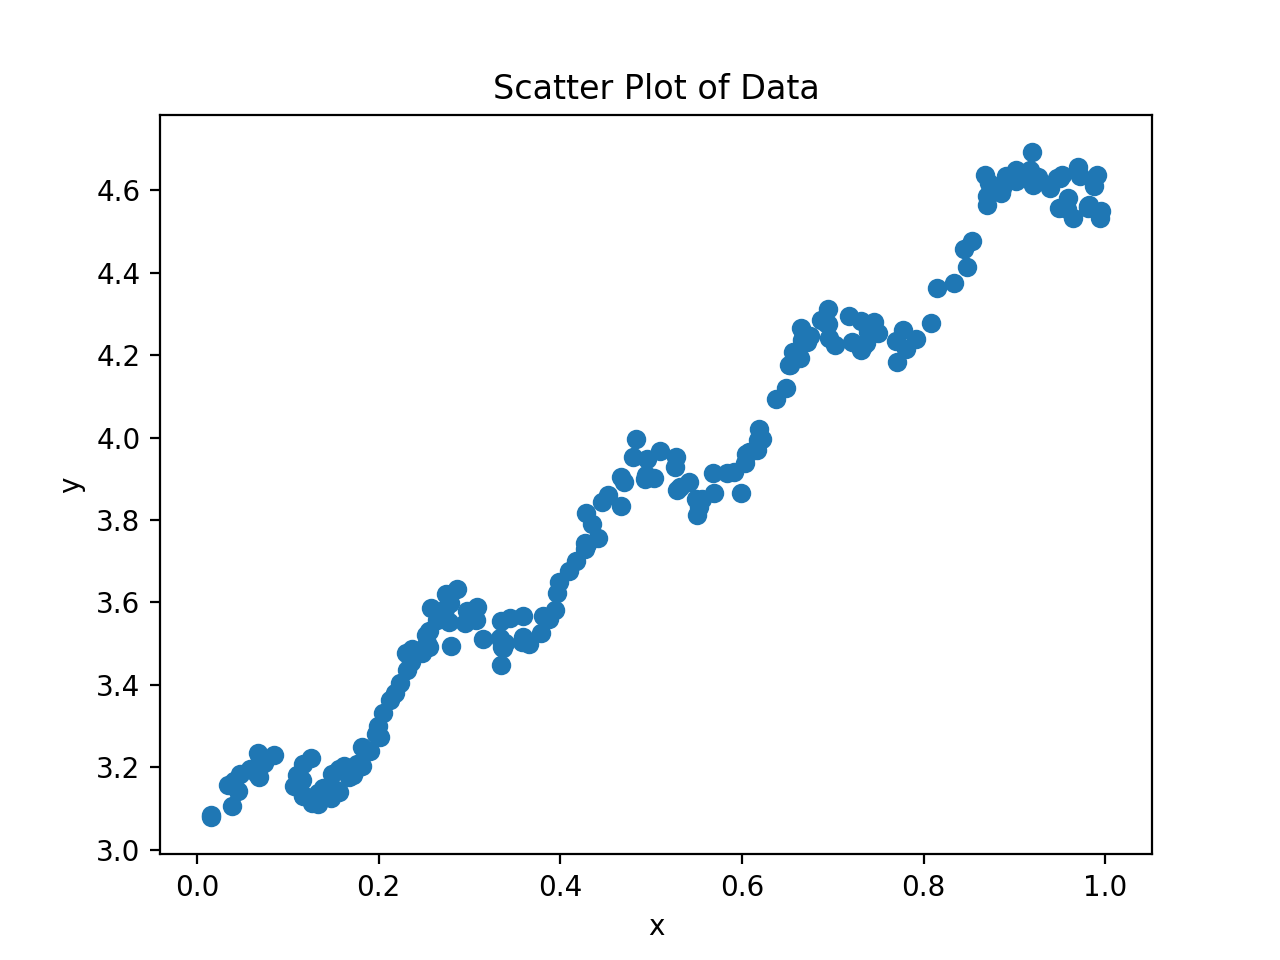
\includegraphics[width=\linewidth]{figures/data.png}
    \end{subfigure}
    \caption{Data Plot}
    \label{fig:data}
\end{figure}

The learned theta of the Normal Equation is $[3.0077,\, 1.6953]$, whose line is shown in Figure \ref{fig:ne}.
\medskip


\begin{figure}[!h]
    \centering
    \begin{subfigure}[b]{0.4\linewidth}
      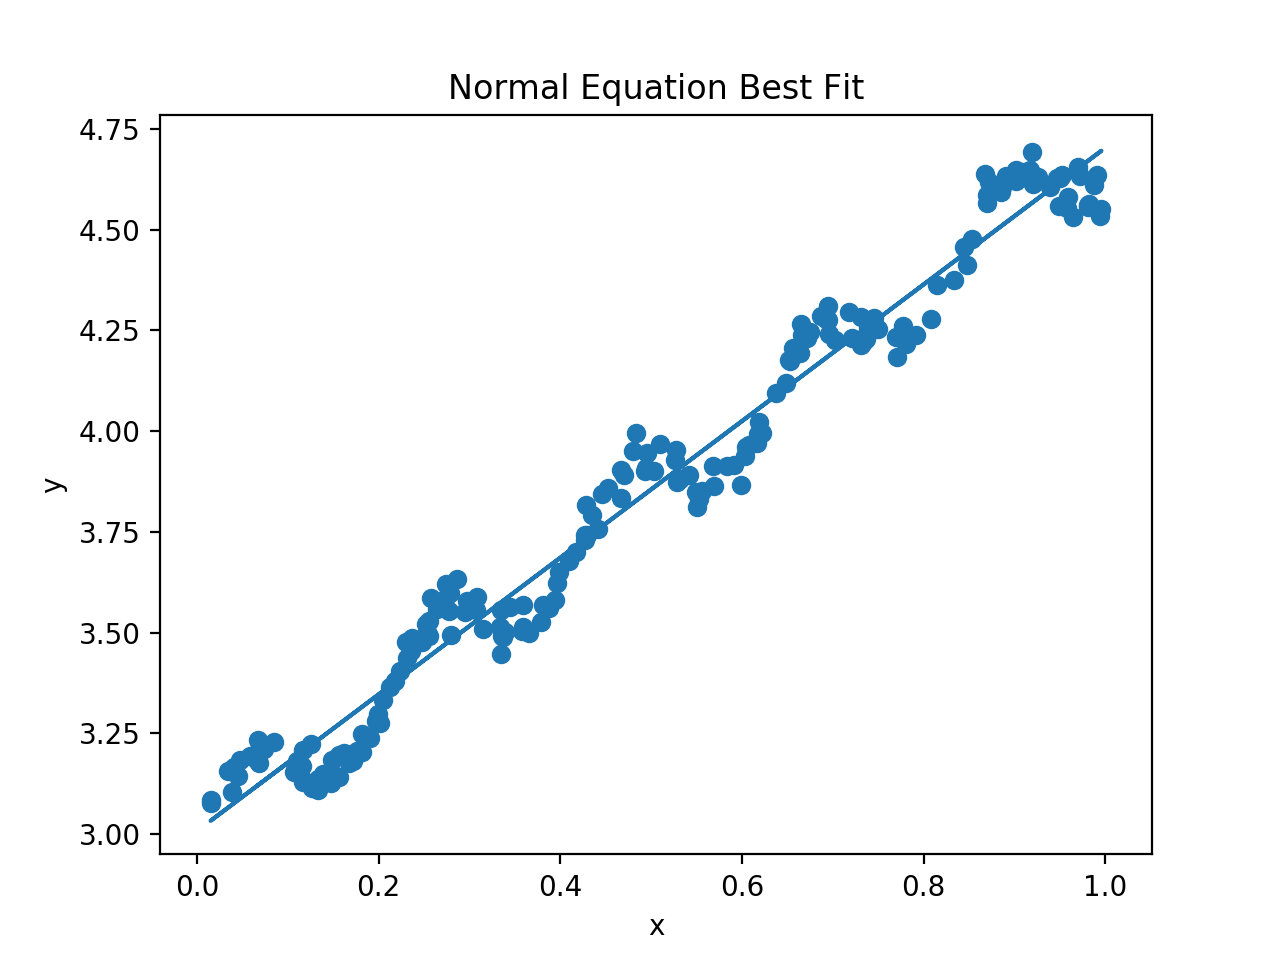
\includegraphics[width=\linewidth]{figures/normal.png}
    \end{subfigure}
    \caption{Normal Equation}
    \label{fig:ne}
\end{figure}

The learned Theta of the Gradient Descent is $[3.0202,\, 1.6715]$ with learning rate of $1e-3$, whose line and loss are shown in Figure \ref{fig:gd}. For the range of learning rate $[0.001,\, 0.005,\, 0.01,\, 0.05,\, 0.1,\, 0.3]$, only smaller ones ($0.001$ and $0.005$) can train the model. With larger learning rates, it will never converge and its training loss keep increasing. This is because in every update, the gradient of the GD model is calculated by summing all the data. Compared with the SGD, the absolute value of the gradient can be much larger which is impacted by the dataset size. Therefore, large learning rates make the theta move to the gradient direction too much which jumps over the optimal value and may land on somewhere with even larger gradient. That's why the large learning rates keep worsening the training loss and we need small rates here.
\medskip


\begin{figure}[!h]
    \centering
    \begin{subfigure}[b]{0.4\linewidth}
      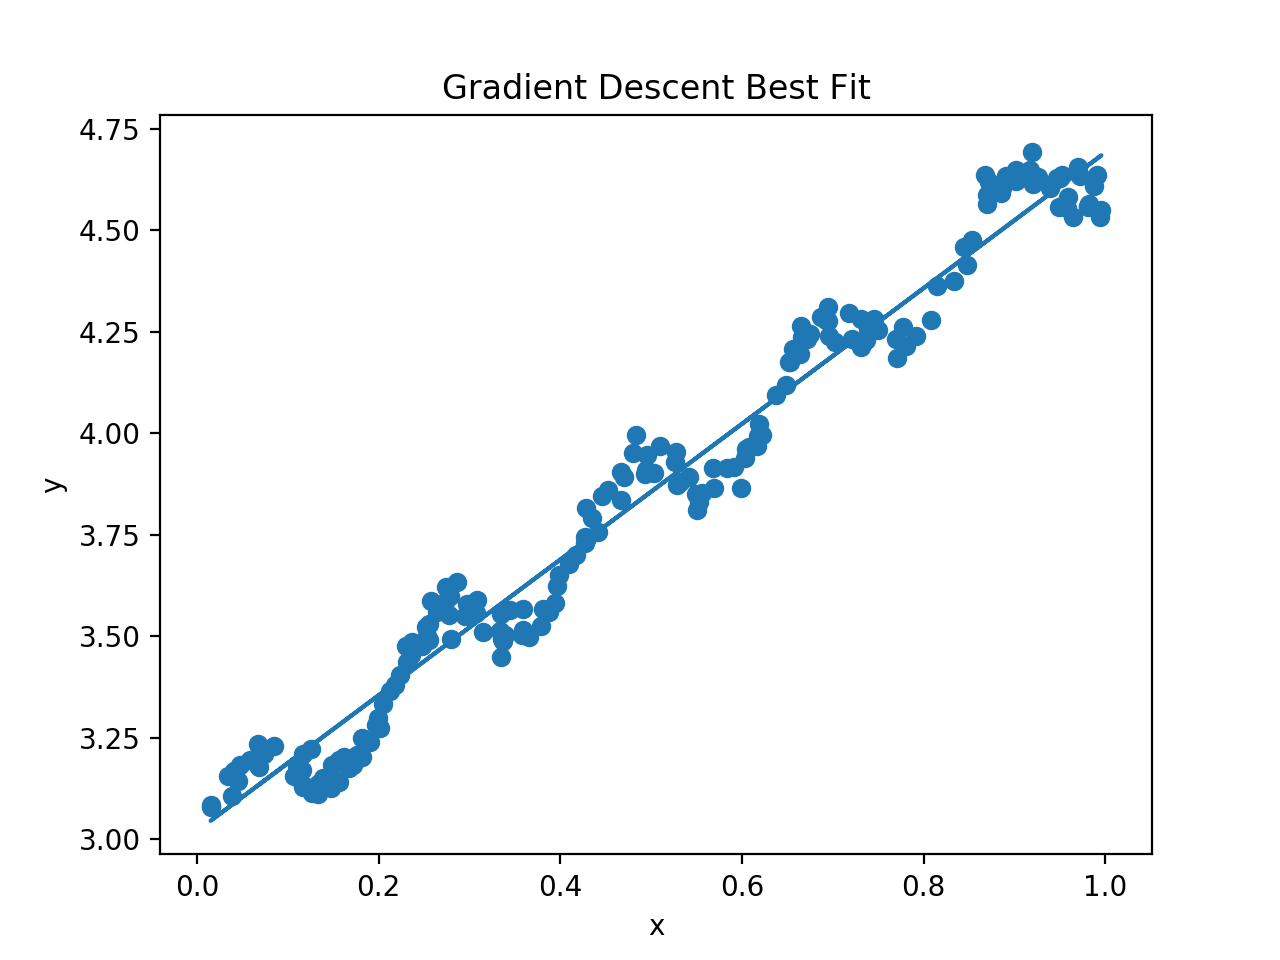
\includegraphics[width=\linewidth]{figures/gd.png}
    \end{subfigure}
    \begin{subfigure}[b]{0.4\linewidth}
      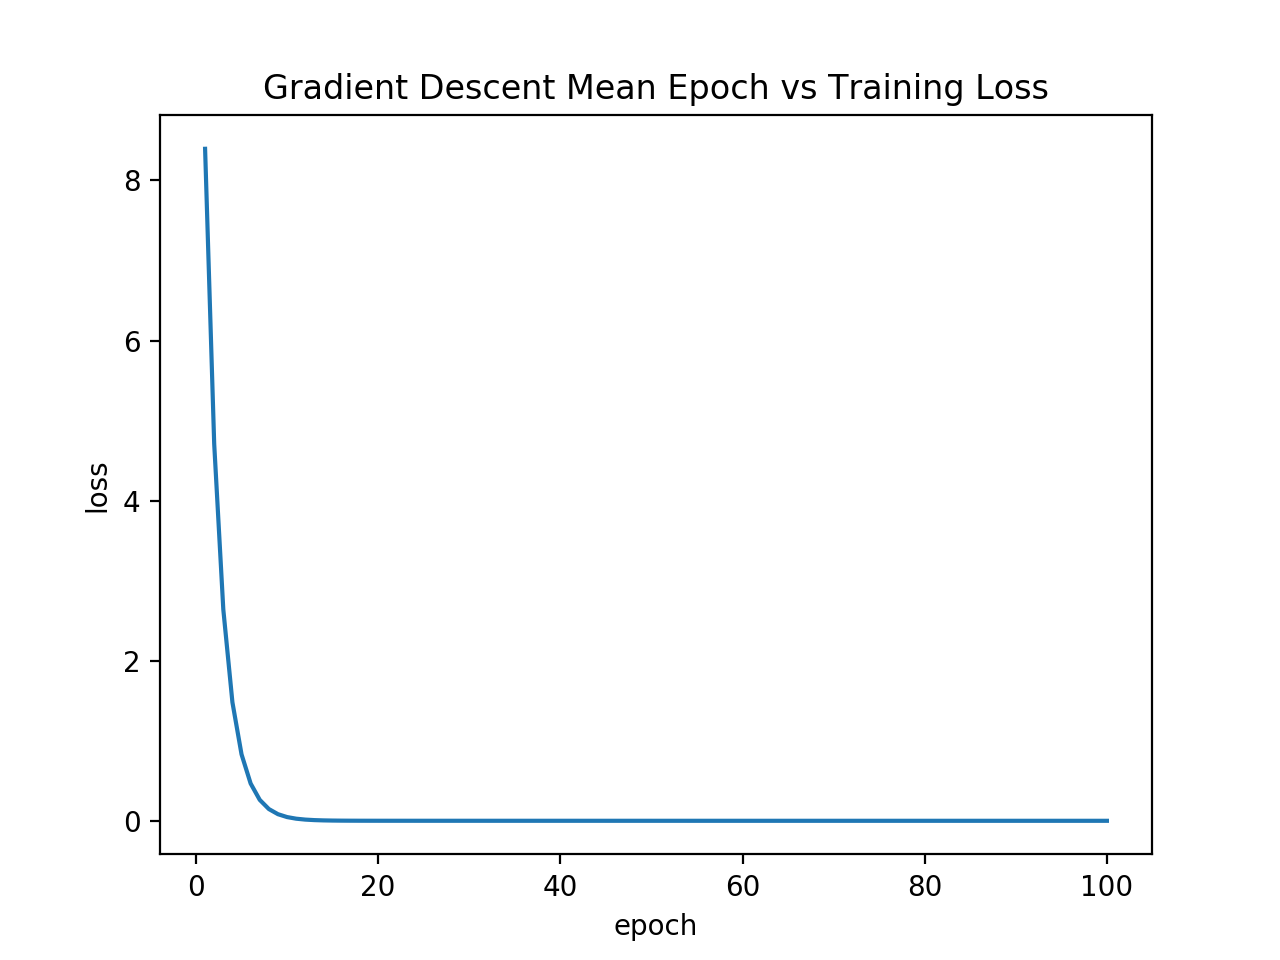
\includegraphics[width=\linewidth]{figures/gd_loss.png}
    \end{subfigure}
    \caption{Gradient Descent}
    \label{fig:gd}
\end{figure}

The learned Theta of the Stochiastic Gradient Descent is $[3.0197,\, 1.6720]$, whose line and loss are shown in Figure \ref{fig:sgd}. For the range of learning rate $[0.001,\, 0.005,\, 0.01,\, 0.05,\, 0.1,\, 0.3]$, all can achieve similarly good training loss in the end, but larger rates converge much faster. In SGD, every update step only calcluate the gradient for one record. The absolute value is quite small, so even the relatively larger rates will not make the step size too large like the GD above. Since they can all reach the optimal points in the end, the larger step size makes the model be there earlier.
\medskip

\begin{figure}[!h]
    \centering
    \begin{subfigure}[b]{0.4\linewidth}
      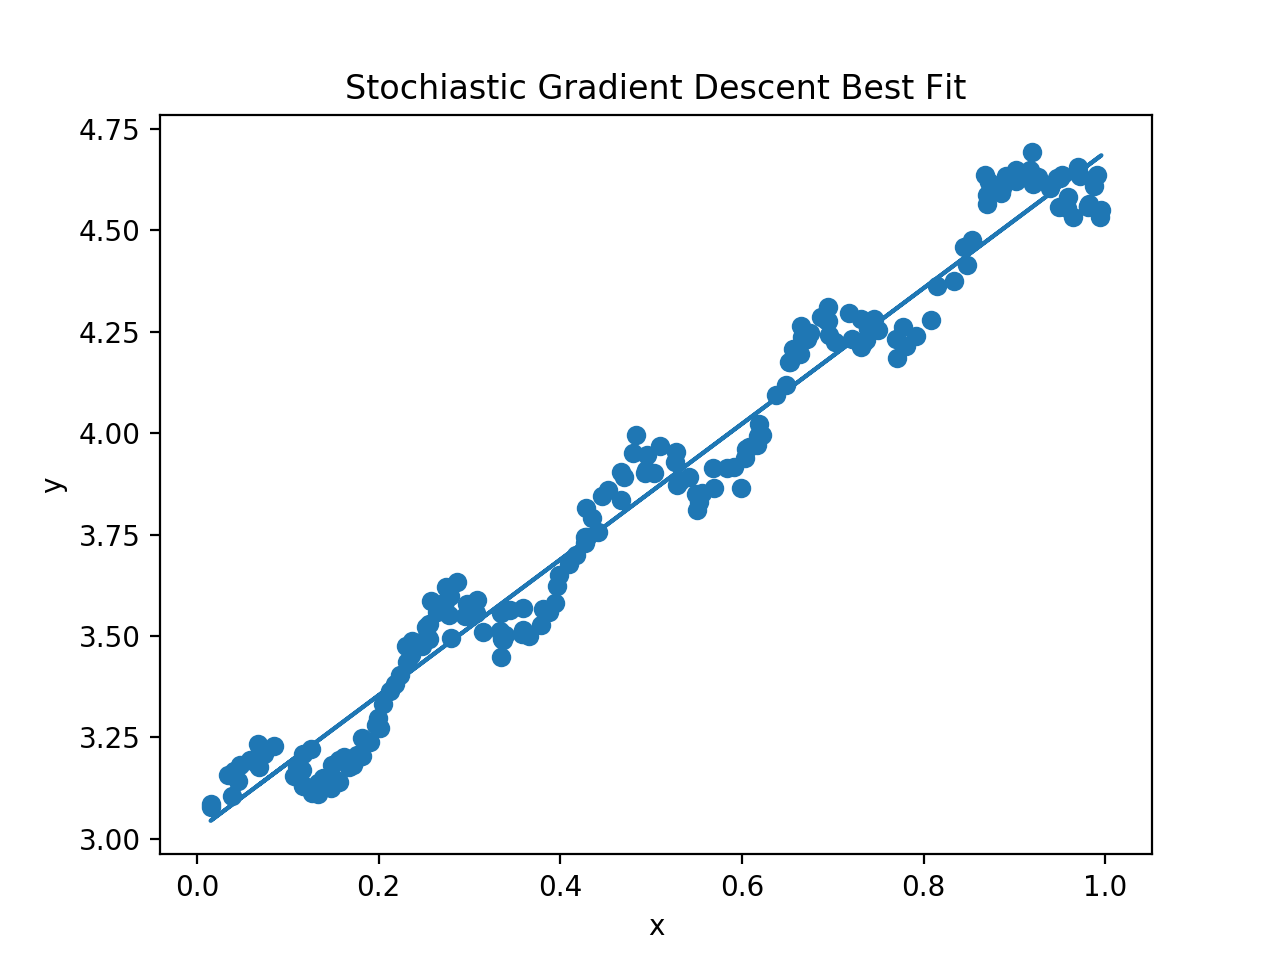
\includegraphics[width=\linewidth]{figures/sgd.png}
    \end{subfigure}
    \begin{subfigure}[b]{0.4\linewidth}
      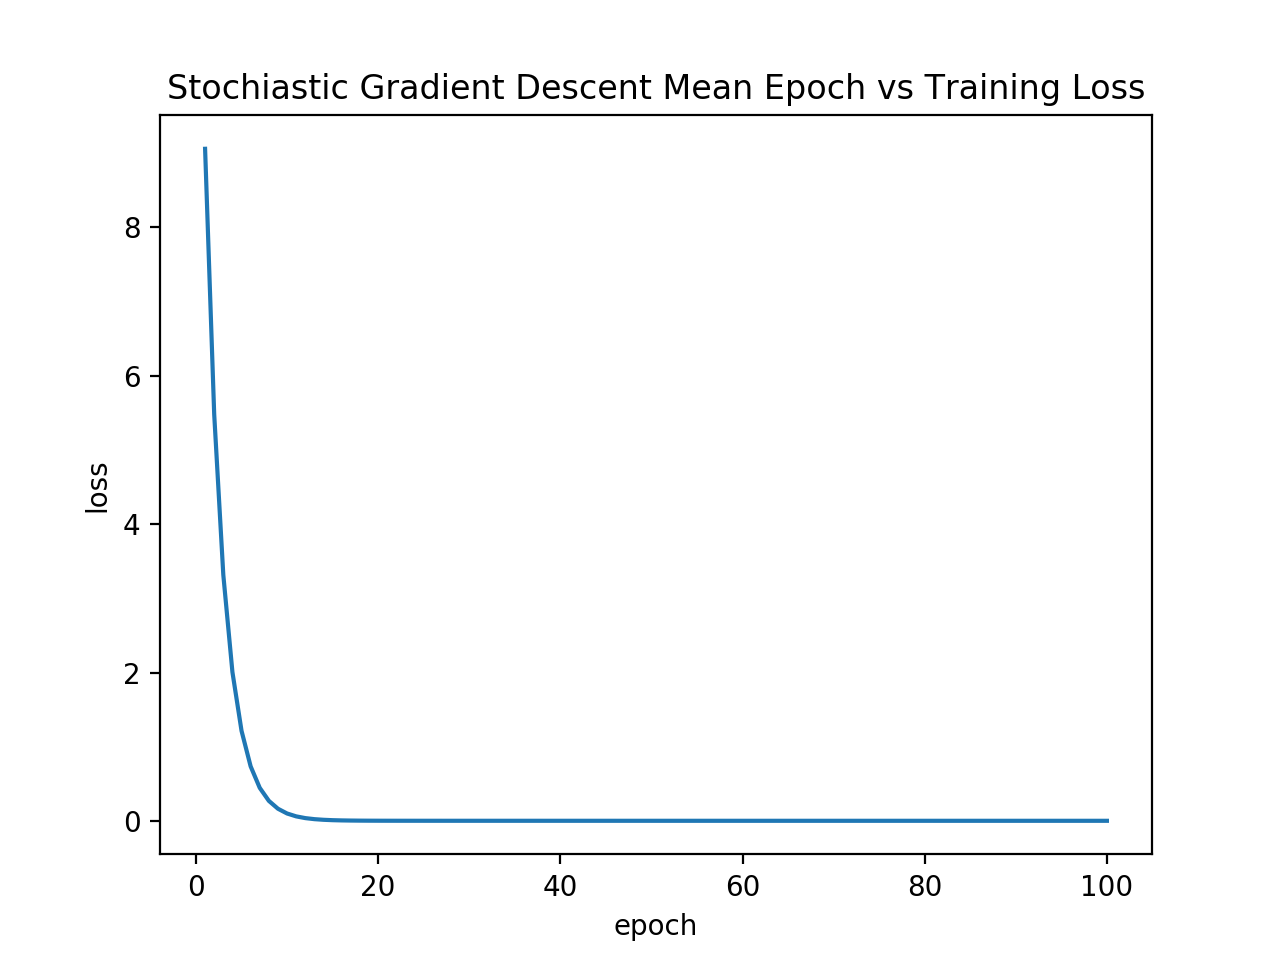
\includegraphics[width=\linewidth]{figures/sgd_loss.png}
    \end{subfigure}
    \caption{Stochiastic Gradient Descent}
    \label{fig:sgd}
\end{figure}

The learned Theta of the Minibatch Gradient Descent is $[3.0204,\, 1.6716]$, whose line and loss are shown in Figure \ref{fig:bsgd}. Different batch sizes lead to different converge rate. I have tested a range of batch sizes $[1,\, 10,\, 20,\, 40,\, 80,\, 100]$. $100$ has the fastest converge rate. Smaller batch sizes make the training progress more like SGD, where the model diverges a lot because the batch gradient direction is far from the optimal direction. The gradient of a larger batch size is closer to the whole training dataset.
\medskip

\begin{figure}[!h]
    \centering
    \begin{subfigure}[b]{0.4\linewidth}
      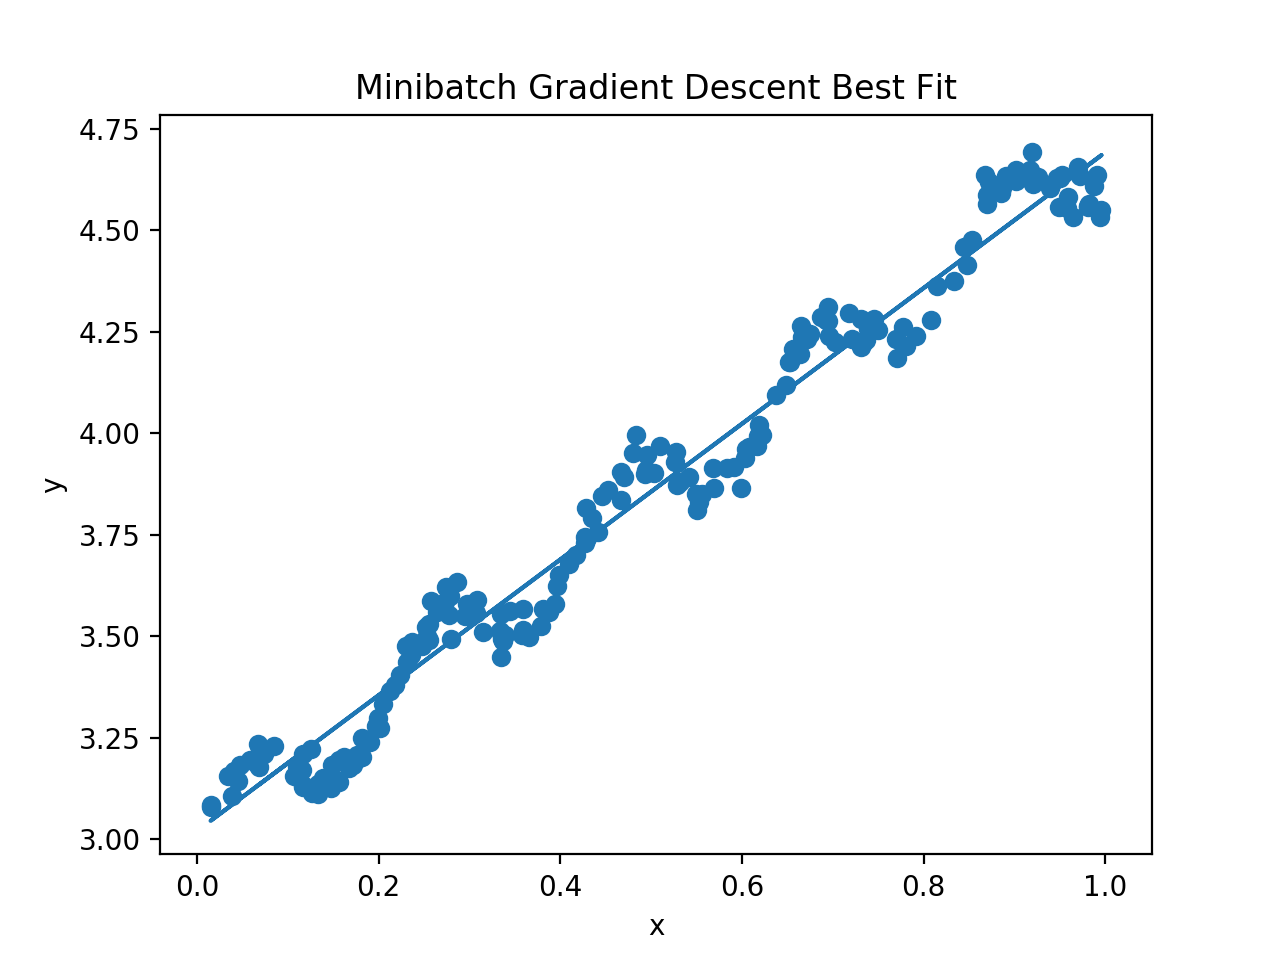
\includegraphics[width=\linewidth]{figures/bsgd.png}
    \end{subfigure}
    \begin{subfigure}[b]{0.4\linewidth}
      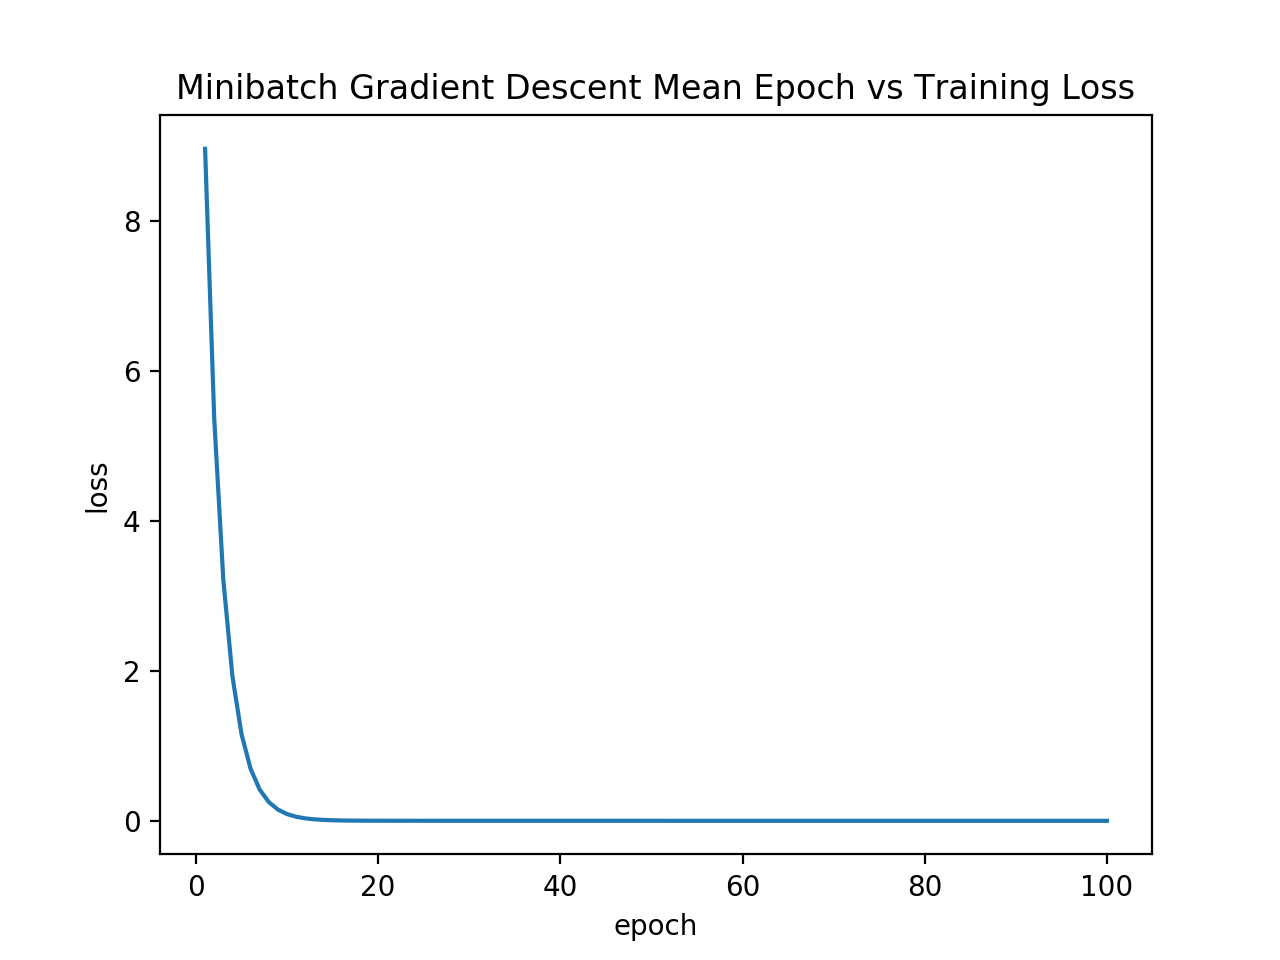
\includegraphics[width=\linewidth]{figures/bsgd_loss.png}
    \end{subfigure}
    \caption{Minibatch Gradient Descent}
    \label{fig:bsgd}
\end{figure}

\item
Sample Exam Questions

3.1

The mean squared training error is $0$

\medskip
3.2

(a)

$$ (1^2 + (\frac{2}{3})^2 + 2^2) / 3 = 1.81 $$

(b)

$$ (1^2 + 0.5^2 + 0.5^2) / 3 = 0.5 $$

(c)

Will choose (b)

\medskip
3.3

(e)

A, because with more training data it becomes harder to well fit all records, it is more likely to make errors.

(f)

B, because more training data can represent the real data distribution better, the left testing data is more likely have been covered in the training.


% ========== Continue adding items as needed

\end{enumerate}

\end{document}
\grid
\grid
